% Options for packages loaded elsewhere
\PassOptionsToPackage{unicode}{hyperref}
\PassOptionsToPackage{hyphens}{url}
%
\documentclass[
]{article}
\title{Explorando os dados traumas}
\author{Felipe}
\date{25/02/2022}

\usepackage{amsmath,amssymb}
\usepackage{lmodern}
\usepackage{iftex}
\ifPDFTeX
  \usepackage[T1]{fontenc}
  \usepackage[utf8]{inputenc}
  \usepackage{textcomp} % provide euro and other symbols
\else % if luatex or xetex
  \usepackage{unicode-math}
  \defaultfontfeatures{Scale=MatchLowercase}
  \defaultfontfeatures[\rmfamily]{Ligatures=TeX,Scale=1}
\fi
% Use upquote if available, for straight quotes in verbatim environments
\IfFileExists{upquote.sty}{\usepackage{upquote}}{}
\IfFileExists{microtype.sty}{% use microtype if available
  \usepackage[]{microtype}
  \UseMicrotypeSet[protrusion]{basicmath} % disable protrusion for tt fonts
}{}
\makeatletter
\@ifundefined{KOMAClassName}{% if non-KOMA class
  \IfFileExists{parskip.sty}{%
    \usepackage{parskip}
  }{% else
    \setlength{\parindent}{0pt}
    \setlength{\parskip}{6pt plus 2pt minus 1pt}}
}{% if KOMA class
  \KOMAoptions{parskip=half}}
\makeatother
\usepackage{xcolor}
\IfFileExists{xurl.sty}{\usepackage{xurl}}{} % add URL line breaks if available
\IfFileExists{bookmark.sty}{\usepackage{bookmark}}{\usepackage{hyperref}}
\hypersetup{
  pdftitle={Explorando os dados traumas},
  pdfauthor={Felipe},
  hidelinks,
  pdfcreator={LaTeX via pandoc}}
\urlstyle{same} % disable monospaced font for URLs
\usepackage[margin=1in]{geometry}
\usepackage{color}
\usepackage{fancyvrb}
\newcommand{\VerbBar}{|}
\newcommand{\VERB}{\Verb[commandchars=\\\{\}]}
\DefineVerbatimEnvironment{Highlighting}{Verbatim}{commandchars=\\\{\}}
% Add ',fontsize=\small' for more characters per line
\usepackage{framed}
\definecolor{shadecolor}{RGB}{248,248,248}
\newenvironment{Shaded}{\begin{snugshade}}{\end{snugshade}}
\newcommand{\AlertTok}[1]{\textcolor[rgb]{0.94,0.16,0.16}{#1}}
\newcommand{\AnnotationTok}[1]{\textcolor[rgb]{0.56,0.35,0.01}{\textbf{\textit{#1}}}}
\newcommand{\AttributeTok}[1]{\textcolor[rgb]{0.77,0.63,0.00}{#1}}
\newcommand{\BaseNTok}[1]{\textcolor[rgb]{0.00,0.00,0.81}{#1}}
\newcommand{\BuiltInTok}[1]{#1}
\newcommand{\CharTok}[1]{\textcolor[rgb]{0.31,0.60,0.02}{#1}}
\newcommand{\CommentTok}[1]{\textcolor[rgb]{0.56,0.35,0.01}{\textit{#1}}}
\newcommand{\CommentVarTok}[1]{\textcolor[rgb]{0.56,0.35,0.01}{\textbf{\textit{#1}}}}
\newcommand{\ConstantTok}[1]{\textcolor[rgb]{0.00,0.00,0.00}{#1}}
\newcommand{\ControlFlowTok}[1]{\textcolor[rgb]{0.13,0.29,0.53}{\textbf{#1}}}
\newcommand{\DataTypeTok}[1]{\textcolor[rgb]{0.13,0.29,0.53}{#1}}
\newcommand{\DecValTok}[1]{\textcolor[rgb]{0.00,0.00,0.81}{#1}}
\newcommand{\DocumentationTok}[1]{\textcolor[rgb]{0.56,0.35,0.01}{\textbf{\textit{#1}}}}
\newcommand{\ErrorTok}[1]{\textcolor[rgb]{0.64,0.00,0.00}{\textbf{#1}}}
\newcommand{\ExtensionTok}[1]{#1}
\newcommand{\FloatTok}[1]{\textcolor[rgb]{0.00,0.00,0.81}{#1}}
\newcommand{\FunctionTok}[1]{\textcolor[rgb]{0.00,0.00,0.00}{#1}}
\newcommand{\ImportTok}[1]{#1}
\newcommand{\InformationTok}[1]{\textcolor[rgb]{0.56,0.35,0.01}{\textbf{\textit{#1}}}}
\newcommand{\KeywordTok}[1]{\textcolor[rgb]{0.13,0.29,0.53}{\textbf{#1}}}
\newcommand{\NormalTok}[1]{#1}
\newcommand{\OperatorTok}[1]{\textcolor[rgb]{0.81,0.36,0.00}{\textbf{#1}}}
\newcommand{\OtherTok}[1]{\textcolor[rgb]{0.56,0.35,0.01}{#1}}
\newcommand{\PreprocessorTok}[1]{\textcolor[rgb]{0.56,0.35,0.01}{\textit{#1}}}
\newcommand{\RegionMarkerTok}[1]{#1}
\newcommand{\SpecialCharTok}[1]{\textcolor[rgb]{0.00,0.00,0.00}{#1}}
\newcommand{\SpecialStringTok}[1]{\textcolor[rgb]{0.31,0.60,0.02}{#1}}
\newcommand{\StringTok}[1]{\textcolor[rgb]{0.31,0.60,0.02}{#1}}
\newcommand{\VariableTok}[1]{\textcolor[rgb]{0.00,0.00,0.00}{#1}}
\newcommand{\VerbatimStringTok}[1]{\textcolor[rgb]{0.31,0.60,0.02}{#1}}
\newcommand{\WarningTok}[1]{\textcolor[rgb]{0.56,0.35,0.01}{\textbf{\textit{#1}}}}
\usepackage{graphicx}
\makeatletter
\def\maxwidth{\ifdim\Gin@nat@width>\linewidth\linewidth\else\Gin@nat@width\fi}
\def\maxheight{\ifdim\Gin@nat@height>\textheight\textheight\else\Gin@nat@height\fi}
\makeatother
% Scale images if necessary, so that they will not overflow the page
% margins by default, and it is still possible to overwrite the defaults
% using explicit options in \includegraphics[width, height, ...]{}
\setkeys{Gin}{width=\maxwidth,height=\maxheight,keepaspectratio}
% Set default figure placement to htbp
\makeatletter
\def\fps@figure{htbp}
\makeatother
\setlength{\emergencystretch}{3em} % prevent overfull lines
\providecommand{\tightlist}{%
  \setlength{\itemsep}{0pt}\setlength{\parskip}{0pt}}
\setcounter{secnumdepth}{-\maxdimen} % remove section numbering
\ifLuaTeX
  \usepackage{selnolig}  % disable illegal ligatures
\fi

\begin{document}
\maketitle

Carregando bibliotecas para manipulação de dados (nem todos foram
utilizados até então)

\begin{verbatim}
## Warning: package 'pastecs' was built under R version 4.1.3
\end{verbatim}

Carregando dados do arquivo ``traumas.csv''

\begin{Shaded}
\begin{Highlighting}[]
\NormalTok{dados\_traumas }\OtherTok{\textless{}{-}} \FunctionTok{read.csv}\NormalTok{(}\StringTok{"traumas.csv"}\NormalTok{, }\AttributeTok{na.strings =} \FunctionTok{c}\NormalTok{(}\StringTok{""}\NormalTok{,}\StringTok{"NA"}\NormalTok{), }\AttributeTok{sep =} \StringTok{";"}\NormalTok{) }
\CommentTok{\#names(dados\_traumas) \#execute este comando para ver os nomes das colunas/variáveis presentes no banco de dados}
\CommentTok{\#View(dados\_traumas) \#execute para visualizar todo o conjunto de dados em uma tabela separada}
\FunctionTok{head}\NormalTok{(dados\_traumas) }
\end{Highlighting}
\end{Shaded}

\begin{verbatim}
##                autor_ano  pais             regiao                    sitio
## 1 Benyon and Siegel 1981  Peru South Peru_Paracas      Santo_Domingo_Pampa
## 2     Standen et al 2020 Chile              Arica    Arica_Acha3C4_Acha3C1
## 3     Standen et al 2020 Chile              Arica Arica_Morro_Praia Miller
## 4     Standen et al 2020 Chile              Arica                    Arica
## 5     Standen et al 2020 Chile              Arica                    Arica
## 6     Standen et al 2010 Chile     Vale de Azapa                    AZ_146
##   long_leste_m lat_sul_m elevacao_m    cultura cronologia data_absBP_.inicial
## 1     365028.4   8467514         17        NID        ARC                8340
## 2     360360.0   7955939         71 Chinchorro        ARC               10000
## 3     360360.0   7955939         71 Chinchorro        ARC                8000
## 4     360360.0   7955939         71 Chinchorro        ARC                6000
## 5     360360.0   7955939         71 Chinchorro        ARC                6000
## 6     375393.0   7951291        278        NID         FF                2740
##   data_absBP_final sexo n_id n_id_traumas sem_traumas fr_traumas
## 1             6220    M    2            0           2       <NA>
## 2             8000    M    4            2           2       0,50
## 3             6000    M   12            3           9       0,25
## 4             4000    M   63           20          43       0,32
## 5             4000    F   57           11          46       0,19
## 6             1930    M    3            3           0       1,00
##   n_id_antimortem fr_antimortem n_id_perimortem fr_perimortem n_tr_anterior
## 1               0          <NA>               0          <NA>             0
## 2               2          0,50               0          <NA>             1
## 3               2          0,17               1          0,08             3
## 4              18          0,29               2          0,03            NA
## 5              11          0,19               0          <NA>            NA
## 6               0          <NA>               3          1,00             3
##   nasal frontal n_tr_posterior n_tr_pariental parietal_e pariental_d
## 1     0       0              0              0          0           0
## 2    NA      NA              0             NA         NA          NA
## 3    NA      NA              0             NA         NA          NA
## 4    NA      NA             NA             NA         NA          NA
## 5    NA      NA             NA             NA         NA          NA
## 6    NA      NA              0             NA         NA          NA
##   n_tr_lateral n_antimortem_lateral n_tr_perimortem_lateral lateral_e lateral_d
## 1            0                   NA                      NA        NA        NA
## 2            1                   NA                      NA        NA        NA
## 3            0                   NA                      NA        NA        NA
## 4           NA                   NA                      NA        NA        NA
## 5           NA                   NA                      NA        NA        NA
## 6            3                   NA                      NA        NA        NA
##   ev_fort estr_sociopolitica   clima carc_geografica
## 1       0               <NA> deserto           costa
## 2       0              Tribo deserto           costa
## 3       0              Tribo deserto           costa
## 4       0              Tribo deserto           costa
## 5       0              Tribo deserto           costa
## 6       0              Tribo deserto            vale
\end{verbatim}

Filtrando dados do Peru que contenha somente os 3 seguintes períodos:
Período Intermédio Primeiro (PIP), Horizonte Médio (HM), e Período
Intermédio Tardio (PIT):

\begin{Shaded}
\begin{Highlighting}[]
\CommentTok{\# usando o operador pipe " \%\textgreater{}\% " da bilioteca tydiverse para manipular os dados:}

\NormalTok{data.tr.peru }\OtherTok{\textless{}{-}}\NormalTok{ dados\_traumas }\SpecialCharTok{\%\textgreater{}\%} \FunctionTok{filter}\NormalTok{(pais}\SpecialCharTok{\%in\%}\FunctionTok{c}\NormalTok{(}\StringTok{"Peru"}\NormalTok{))}\SpecialCharTok{\%\textgreater{}\%} \FunctionTok{slice}\NormalTok{(}\SpecialCharTok{{-}}\DecValTok{1}\NormalTok{) }\CommentTok{\#a função slice é usada para remover a primeira linha que continha um dado do Arcaico}
                                           
\CommentTok{\#View(data.tr.peru)}
\CommentTok{\#names(data.tr.peru)}
\FunctionTok{head}\NormalTok{(data.tr.peru)}
\end{Highlighting}
\end{Shaded}

\begin{verbatim}
##                         autor_ano pais   regiao      sitio long_leste_m
## 1           Tung 2007 e Tung 2012 Peru Ayacucho Conchopata     579248.9
## 2           Tung 2007 e Tung 2012 Peru Ayacucho Conchopata     579248.9
## 3           Tung 2007 e Tung 2012 Peru Ayacucho Conchopata     579248.9
## 4 Tung 2007, Tung 2012, Tung 2008 Peru Ayacucho Conchopata     579248.9
## 5           Tung 2007 e Tung 2012 Peru Ayacucho Conchopata     579248.9
## 6           Tung 2007 e Tung 2012 Peru Ayacucho Conchopata     579248.9
##   lat_sul_m elevacao_m         cultura cronologia data_absBP_.inicial
## 1   8545412       2839 Pré_Wari_Huarpa        PIP                1700
## 2   8545412       2839 Pré_Wari_Huarpa        PIP                1700
## 3   8545412       2839 Pré_Wari_Huarpa        PIP                1700
## 4   8545412       2839            Wari         HM                1300
## 5   8545412       2839            Wari         HM                1300
## 6   8545412       2839            Wari         HM                1300
##   data_absBP_final sexo n_id n_id_traumas sem_traumas fr_traumas
## 1             1350    M    1            1           0       1,00
## 2             1350    F    4            2           2       0,50
## 3             1350  NID    6            0           6       0,00
## 4             1150    M   14            4          10       0,29
## 5             1150    F   25            6          19       0,24
## 6             1150  NID    5            0           5       0,00
##   n_id_antimortem fr_antimortem n_id_perimortem fr_perimortem n_tr_anterior
## 1               1          1,00               0          <NA>             0
## 2               2          0,50               0          <NA>             0
## 3               0          0,00               0          <NA>             0
## 4               4          0,29               0          <NA>             2
## 5               6          0,24               0          <NA>             0
## 6               0          <NA>               0          <NA>             0
##   nasal frontal n_tr_posterior n_tr_pariental parietal_e pariental_d
## 1     0       0              0              0          0           0
## 2     0       0              0              0          0           0
## 3     0       0              0              0          0           0
## 4    NA      NA              4             NA         NA          NA
## 5    NA      NA              7             NA         NA          NA
## 6     0       0              0              0          0           0
##   n_tr_lateral n_antimortem_lateral n_tr_perimortem_lateral lateral_e lateral_d
## 1            1                   NA                      NA        NA        NA
## 2            0                   NA                      NA        NA        NA
## 3            0                   NA                      NA        NA        NA
## 4           NA                   NA                      NA        NA        NA
## 5           NA                   NA                      NA        NA        NA
## 6            0                   NA                      NA        NA        NA
##   ev_fort estr_sociopolitica            clima carc_geografica
## 1       0               <NA> frio_de_montanha            vale
## 2       0               <NA> frio_de_montanha            vale
## 3       0               <NA> frio_de_montanha            vale
## 4       0             Estado frio_de_montanha            vale
## 5       0             Estado frio_de_montanha            vale
## 6       0             Estado frio_de_montanha            vale
\end{verbatim}

'\,'`\# Descrição estatística dos dados:''\,' Realizando descrião
estatítica dos dados númericos de interesse do estudo pela biblioteca
'\,'\,' pastecs '\,'\,'

\begin{Shaded}
\begin{Highlighting}[]
\CommentTok{\#install.packages("pastecs") \# execute para }

\CommentTok{\# realizando descrião estatítica dos dados númericos de interesse do estudo pela biblioteca \textquotesingle{}\textquotesingle{}\textquotesingle{} pastecs \textquotesingle{}\textquotesingle{}\textquotesingle{}}

\CommentTok{\# n\_id = número de individuos, n\_id\_traumas = número de indivíduos com traumas, sem\_traumas = número de indíviduos sem traumas, n\_id\_antimortem = número de indivíduos com traumas antimortem, n\_id\_perimortem = número de indivíduos com traumas perimortem}

\NormalTok{data\_descr }\OtherTok{\textless{}{-}}\NormalTok{ data.tr.peru }\SpecialCharTok{\%\textgreater{}\%} \FunctionTok{select}\NormalTok{(n\_id,n\_id\_traumas,sem\_traumas,n\_id\_antimortem,n\_id\_perimortem)}

\NormalTok{descr }\OtherTok{\textless{}{-}} \FunctionTok{stat.desc}\NormalTok{(data\_descr)}
\FunctionTok{round}\NormalTok{(descr,}\DecValTok{2}\NormalTok{)}
\end{Highlighting}
\end{Shaded}

\begin{verbatim}
##                n_id n_id_traumas sem_traumas n_id_antimortem n_id_perimortem
## nbr.val       36.00        36.00       37.00           26.00           27.00
## nbr.null       1.00         5.00        5.00            6.00           13.00
## nbr.na         1.00         1.00        0.00           11.00           10.00
## min            0.00         0.00        0.00            0.00            0.00
## max          104.00        52.00       72.00           48.00            9.00
## range        104.00        52.00       72.00           48.00            9.00
## sum          853.00       387.00      466.00          212.00           53.00
## median        15.50         6.00        7.00            4.00            1.00
## mean          23.69        10.75       12.59            8.15            1.96
## SE.mean        3.95         2.21        2.30            2.26            0.51
## CI.mean.0.95   8.03         4.49        4.66            4.65            1.04
## var          562.62       176.42      195.41          132.46            6.96
## std.dev       23.72        13.28       13.98           11.51            2.64
## coef.var       1.00         1.24        1.11            1.41            1.34
\end{verbatim}

\begin{Shaded}
\begin{Highlighting}[]
\FunctionTok{library}\NormalTok{(ggplot2)}
\NormalTok{data.tr.peru }\SpecialCharTok{\%\textgreater{}\%} \FunctionTok{filter}\NormalTok{(}\SpecialCharTok{!}\FunctionTok{is.na}\NormalTok{(n\_id))}\SpecialCharTok{\%\textgreater{}\%}
                \FunctionTok{group\_by}\NormalTok{(cronologia) }\SpecialCharTok{\%\textgreater{}\%}\NormalTok{ ggplot}\SpecialCharTok{+}\FunctionTok{geom\_boxplot}\NormalTok{(}\FunctionTok{aes}\NormalTok{(}\AttributeTok{x=}\NormalTok{cronologia,}\AttributeTok{y=}\NormalTok{n\_id))}
\end{Highlighting}
\end{Shaded}

\includegraphics{data.trauma.explorer_files/figure-latex/unnamed-chunk-5-1.pdf}

\begin{Shaded}
\begin{Highlighting}[]
\CommentTok{\#falta alterar títulos e aparência }
\end{Highlighting}
\end{Shaded}

\begin{Shaded}
\begin{Highlighting}[]
\NormalTok{data.tr.peru }\SpecialCharTok{\%\textgreater{}\%} \FunctionTok{filter}\NormalTok{(}\SpecialCharTok{!}\FunctionTok{is.na}\NormalTok{(n\_id\_traumas))}\SpecialCharTok{\%\textgreater{}\%}
                \FunctionTok{group\_by}\NormalTok{(cronologia) }\SpecialCharTok{\%\textgreater{}\%}\NormalTok{ ggplot}\SpecialCharTok{+}\FunctionTok{geom\_boxplot}\NormalTok{(}\FunctionTok{aes}\NormalTok{(}\AttributeTok{x=}\NormalTok{cronologia,}\AttributeTok{y=}\NormalTok{n\_id\_traumas))}
\end{Highlighting}
\end{Shaded}

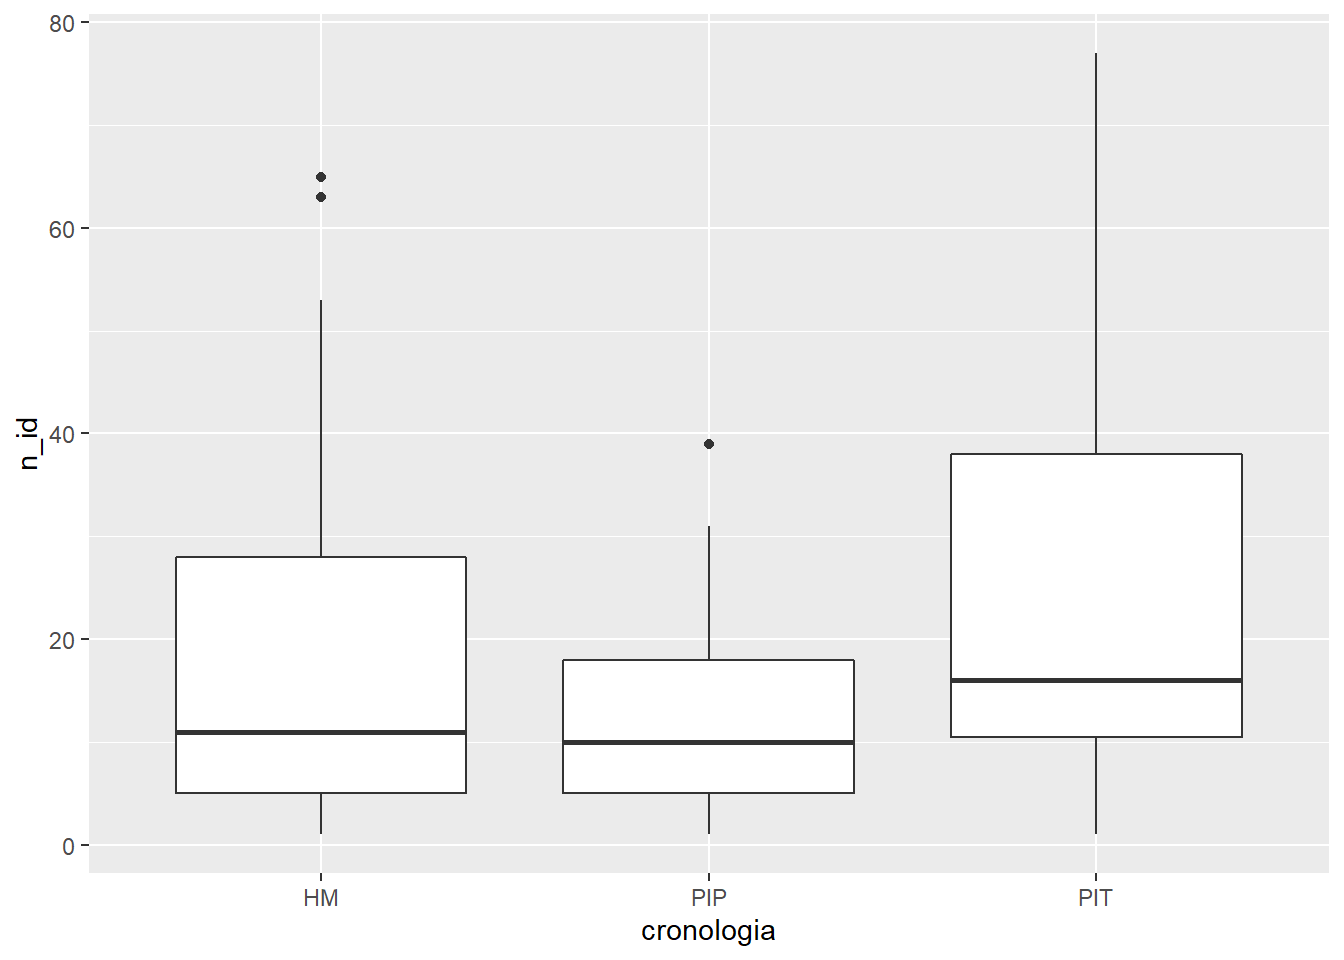
\includegraphics{data.trauma.explorer_files/figure-latex/unnamed-chunk-6-1.pdf}

\begin{Shaded}
\begin{Highlighting}[]
\NormalTok{data.tr.peru }\SpecialCharTok{\%\textgreater{}\%} \FunctionTok{filter}\NormalTok{(}\SpecialCharTok{!}\FunctionTok{is.na}\NormalTok{(n\_id\_antimortem))}\SpecialCharTok{\%\textgreater{}\%}
                \FunctionTok{group\_by}\NormalTok{(cronologia) }\SpecialCharTok{\%\textgreater{}\%}\NormalTok{ ggplot}\SpecialCharTok{+}\FunctionTok{geom\_boxplot}\NormalTok{(}\FunctionTok{aes}\NormalTok{(}\AttributeTok{x=}\NormalTok{cronologia,}\AttributeTok{y=}\NormalTok{n\_id\_antimortem))}
\end{Highlighting}
\end{Shaded}

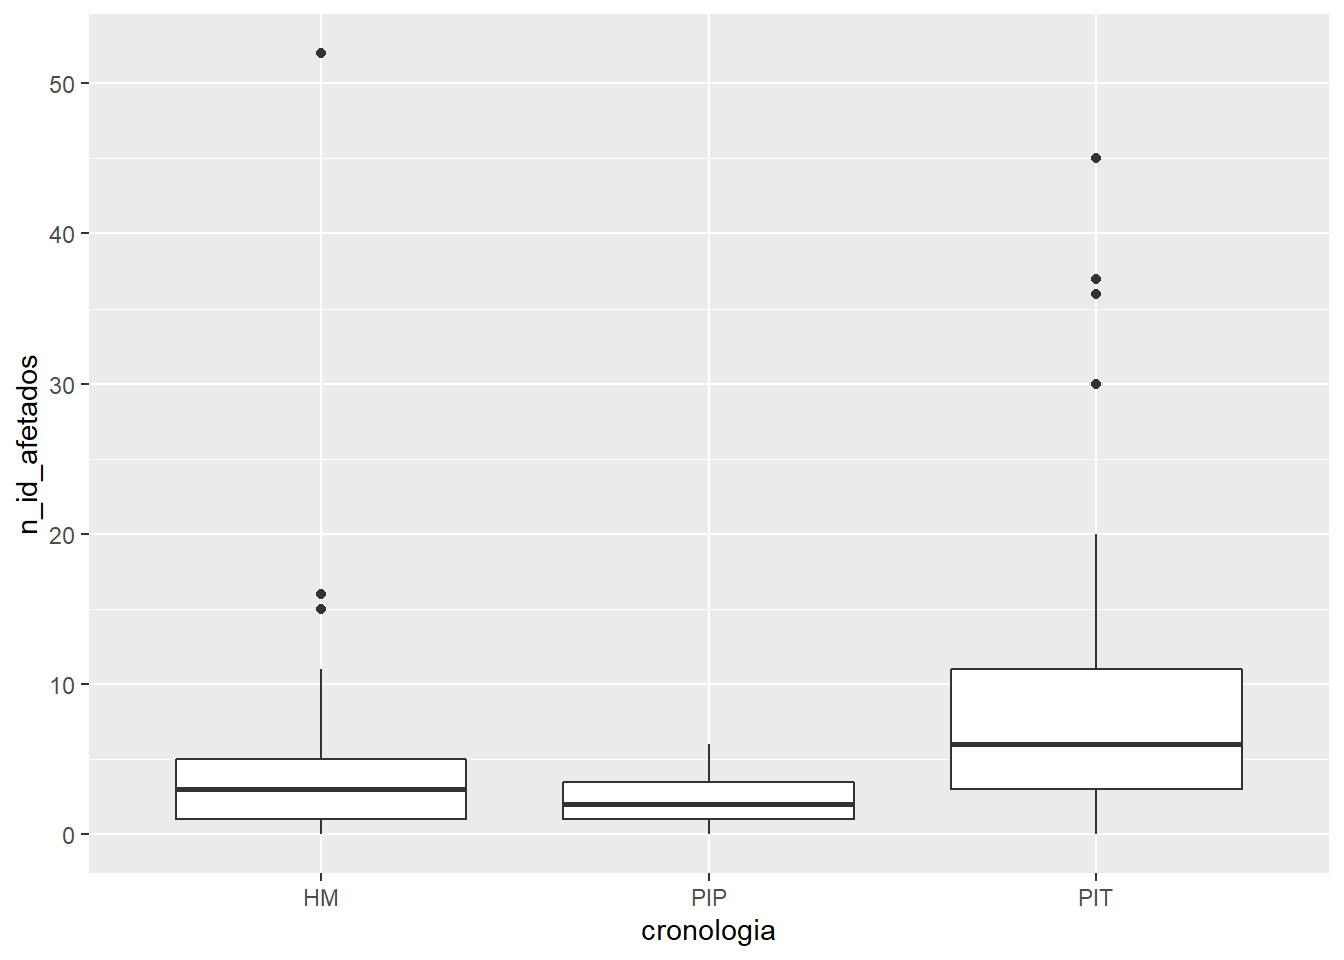
\includegraphics{data.trauma.explorer_files/figure-latex/unnamed-chunk-7-1.pdf}

\begin{Shaded}
\begin{Highlighting}[]
\NormalTok{data.tr.peru }\SpecialCharTok{\%\textgreater{}\%} \FunctionTok{filter}\NormalTok{(}\SpecialCharTok{!}\FunctionTok{is.na}\NormalTok{(n\_id\_perimortem))}\SpecialCharTok{\%\textgreater{}\%}
                \FunctionTok{group\_by}\NormalTok{(cronologia) }\SpecialCharTok{\%\textgreater{}\%}\NormalTok{ ggplot}\SpecialCharTok{+}\FunctionTok{geom\_boxplot}\NormalTok{(}\FunctionTok{aes}\NormalTok{(}\AttributeTok{x=}\NormalTok{cronologia,}\AttributeTok{y=}\NormalTok{n\_id\_perimortem))}
\end{Highlighting}
\end{Shaded}

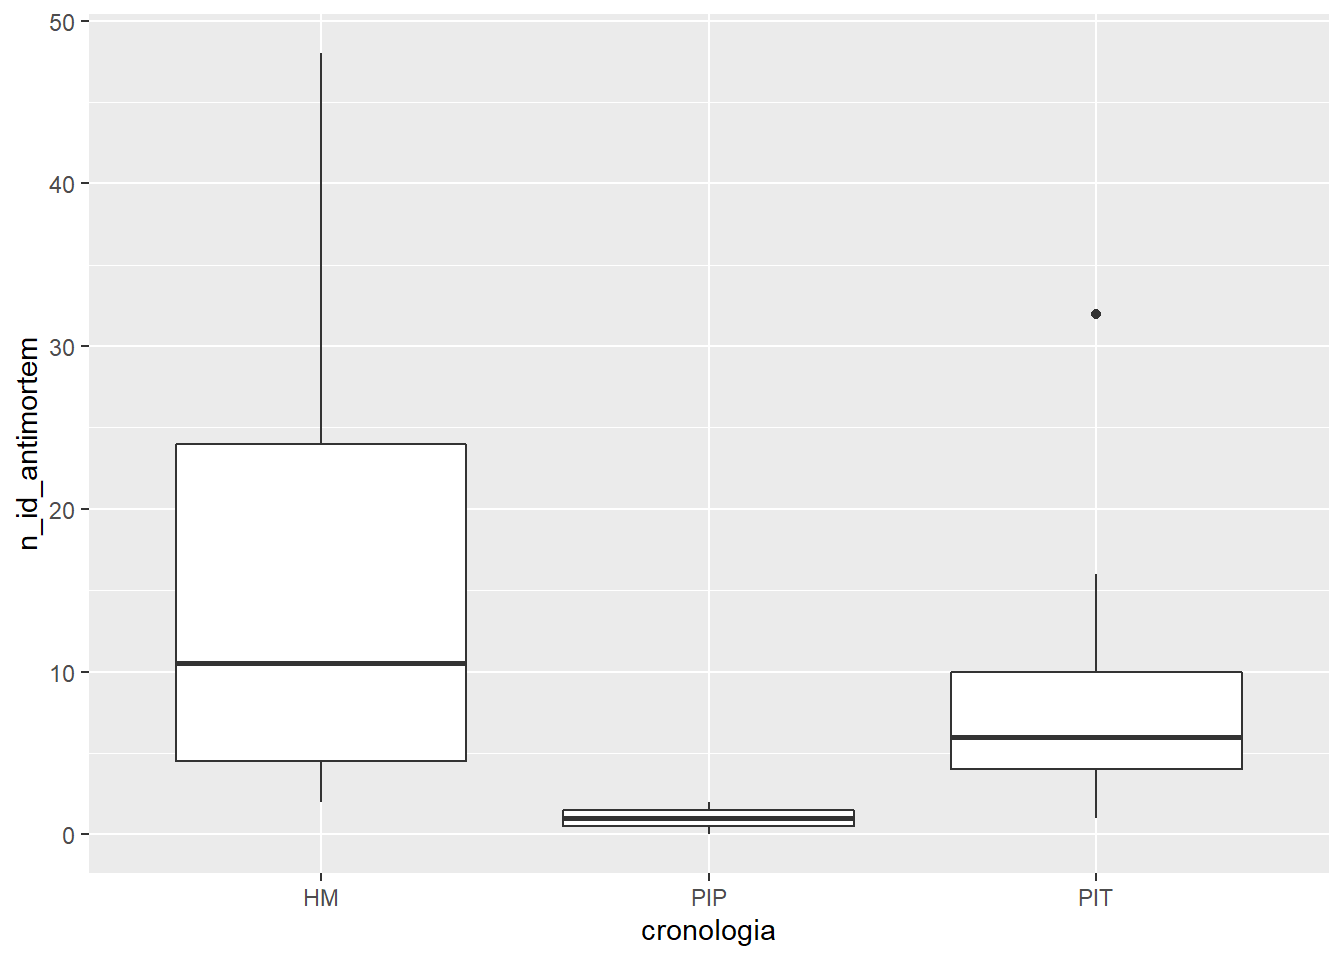
\includegraphics{data.trauma.explorer_files/figure-latex/unnamed-chunk-8-1.pdf}

\begin{Shaded}
\begin{Highlighting}[]
\NormalTok{data.tr.peru }\SpecialCharTok{\%\textgreater{}\%} \FunctionTok{filter}\NormalTok{(}\SpecialCharTok{!}\FunctionTok{is.na}\NormalTok{(n\_id))}\SpecialCharTok{\%\textgreater{}\%}
                \FunctionTok{group\_by}\NormalTok{(sexo) }\SpecialCharTok{\%\textgreater{}\%}\NormalTok{  ggplot}\SpecialCharTok{+}\FunctionTok{geom\_boxplot}\NormalTok{(}\FunctionTok{aes}\NormalTok{(}\AttributeTok{x=}\NormalTok{sexo,}\AttributeTok{y=}\NormalTok{n\_id))}
\end{Highlighting}
\end{Shaded}

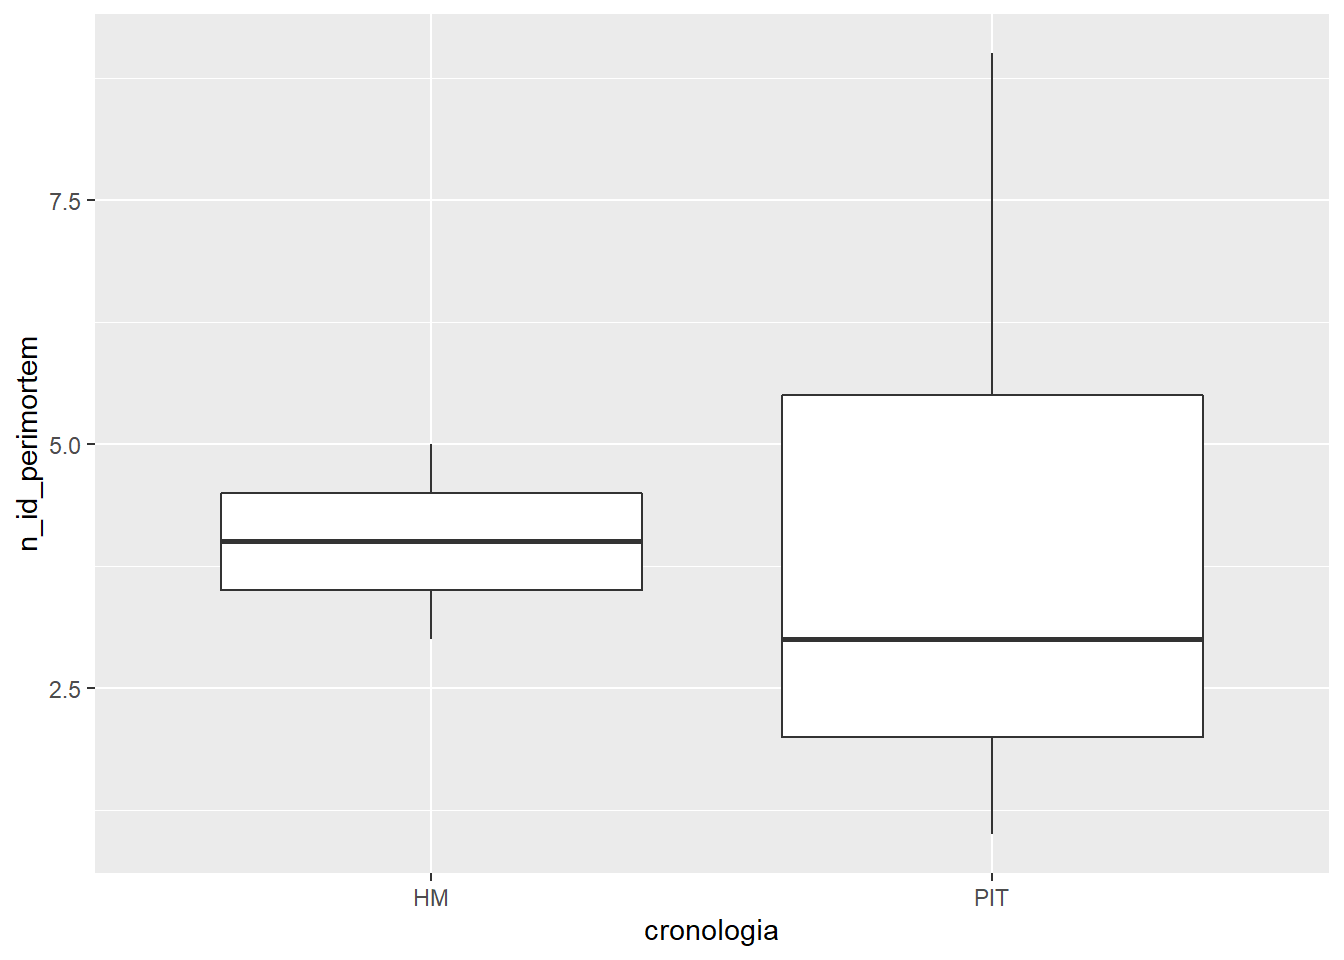
\includegraphics{data.trauma.explorer_files/figure-latex/unnamed-chunk-9-1.pdf}

\begin{Shaded}
\begin{Highlighting}[]
\NormalTok{data.tr.peru }\SpecialCharTok{\%\textgreater{}\%} \FunctionTok{filter}\NormalTok{(}\SpecialCharTok{!}\FunctionTok{is.na}\NormalTok{(n\_id\_traumas))}\SpecialCharTok{\%\textgreater{}\%}
                \FunctionTok{group\_by}\NormalTok{(sexo) }\SpecialCharTok{\%\textgreater{}\%}\NormalTok{  ggplot}\SpecialCharTok{+}\FunctionTok{geom\_boxplot}\NormalTok{(}\FunctionTok{aes}\NormalTok{(}\AttributeTok{x=}\NormalTok{sexo,}\AttributeTok{y=}\NormalTok{n\_id\_traumas))}
\end{Highlighting}
\end{Shaded}

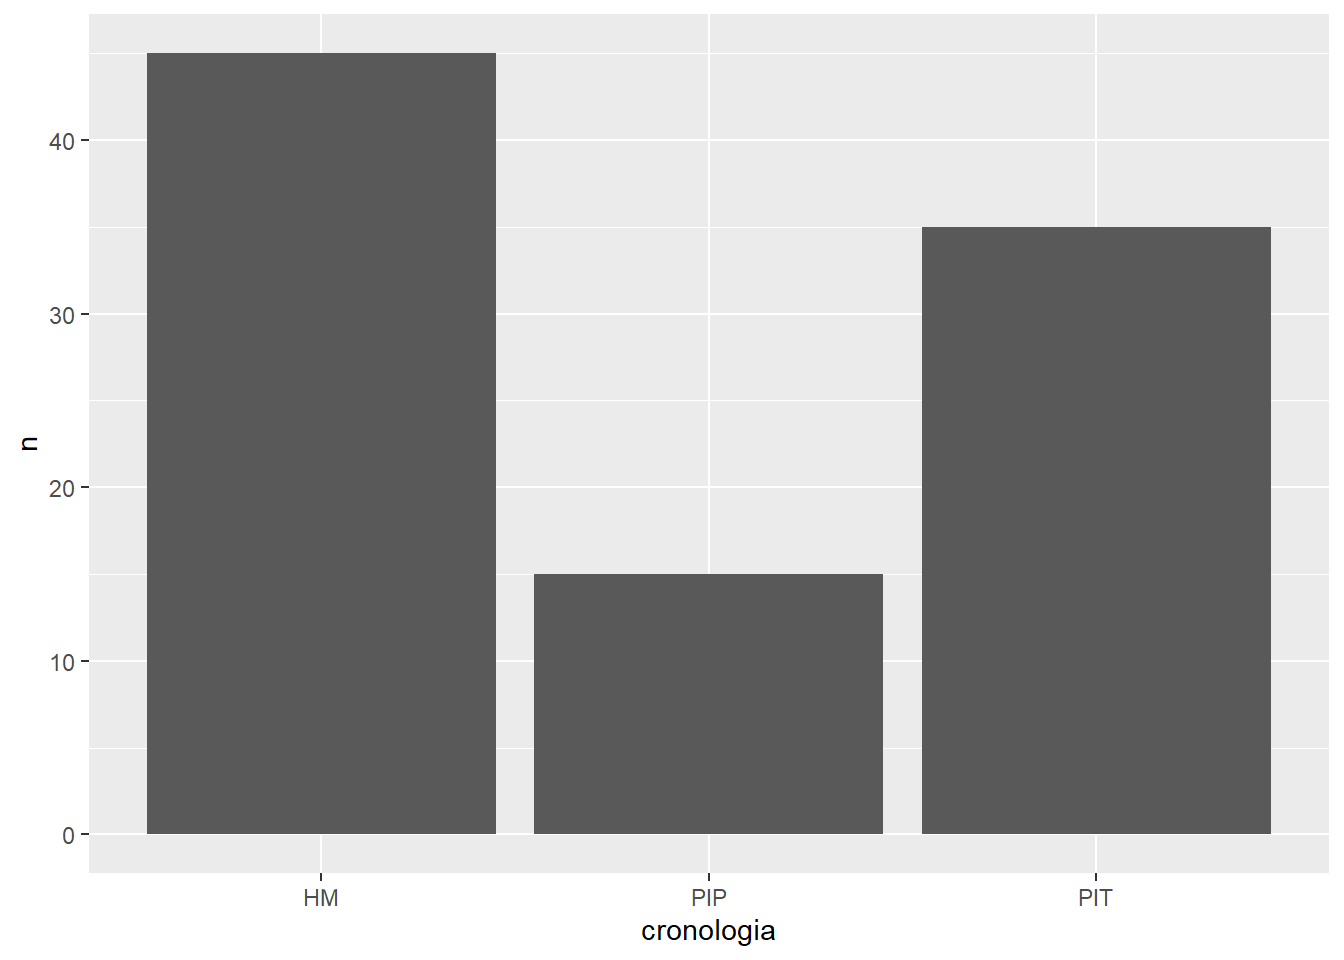
\includegraphics{data.trauma.explorer_files/figure-latex/unnamed-chunk-10-1.pdf}

\begin{Shaded}
\begin{Highlighting}[]
\NormalTok{data.tr.peru }\SpecialCharTok{\%\textgreater{}\%} \FunctionTok{filter}\NormalTok{(}\SpecialCharTok{!}\FunctionTok{is.na}\NormalTok{(n\_id\_antimortem))}\SpecialCharTok{\%\textgreater{}\%}
                \FunctionTok{group\_by}\NormalTok{(sexo) }\SpecialCharTok{\%\textgreater{}\%}\NormalTok{  ggplot}\SpecialCharTok{+}\FunctionTok{geom\_boxplot}\NormalTok{(}\FunctionTok{aes}\NormalTok{(}\AttributeTok{x=}\NormalTok{sexo,}\AttributeTok{y=}\NormalTok{n\_id\_antimortem))}
\end{Highlighting}
\end{Shaded}

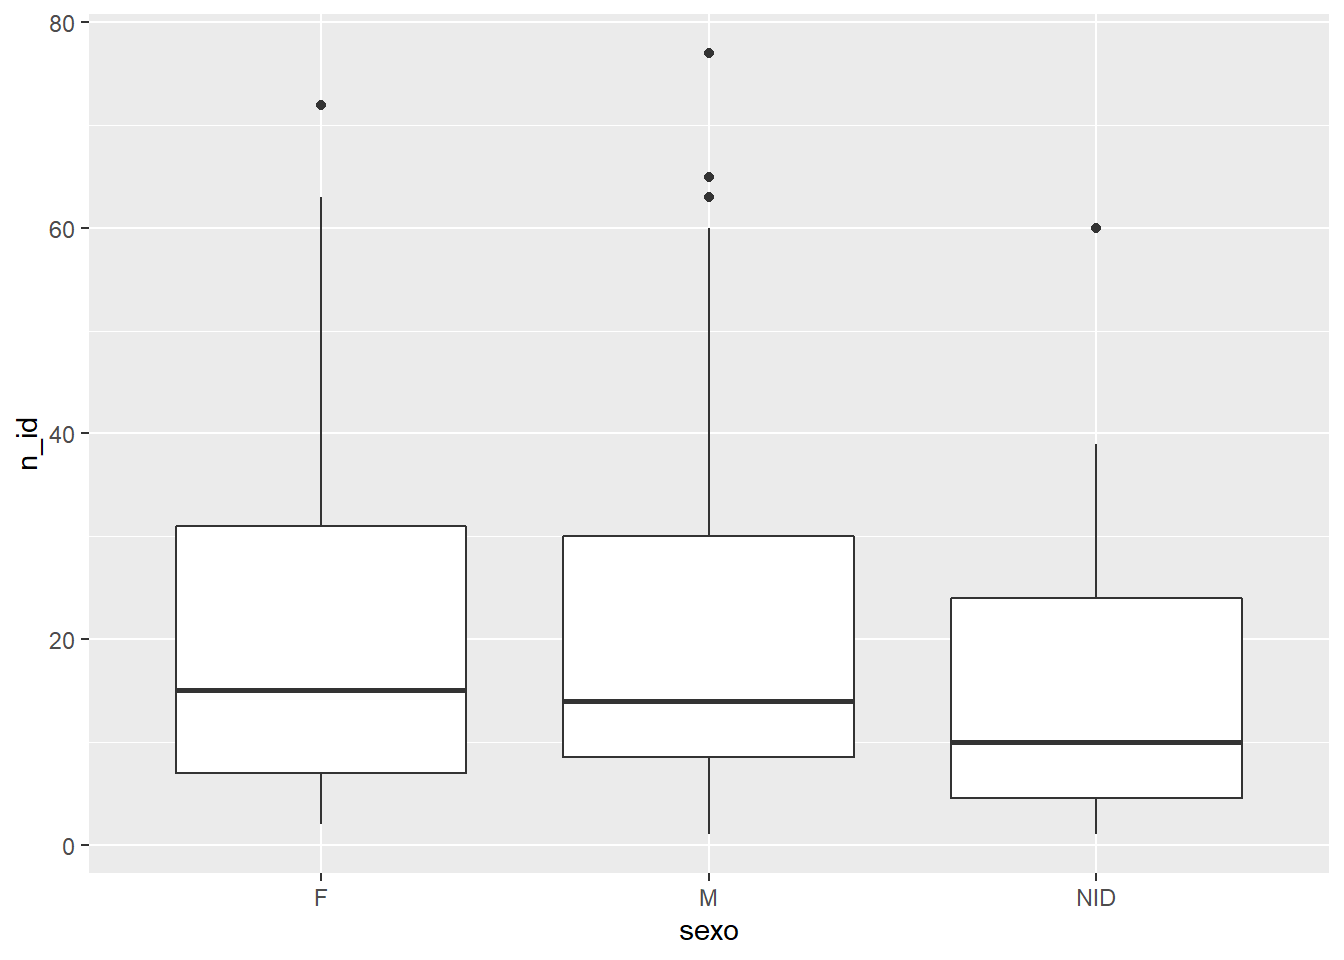
\includegraphics{data.trauma.explorer_files/figure-latex/unnamed-chunk-11-1.pdf}

\begin{Shaded}
\begin{Highlighting}[]
\NormalTok{data.tr.peru }\SpecialCharTok{\%\textgreater{}\%} \FunctionTok{filter}\NormalTok{(}\SpecialCharTok{!}\FunctionTok{is.na}\NormalTok{(n\_id\_perimortem))}\SpecialCharTok{\%\textgreater{}\%}
                \FunctionTok{group\_by}\NormalTok{(sexo) }\SpecialCharTok{\%\textgreater{}\%}\NormalTok{  ggplot}\SpecialCharTok{+}\FunctionTok{geom\_boxplot}\NormalTok{(}\FunctionTok{aes}\NormalTok{(}\AttributeTok{x=}\NormalTok{sexo,}\AttributeTok{y=}\NormalTok{n\_id\_perimortem))}
\end{Highlighting}
\end{Shaded}

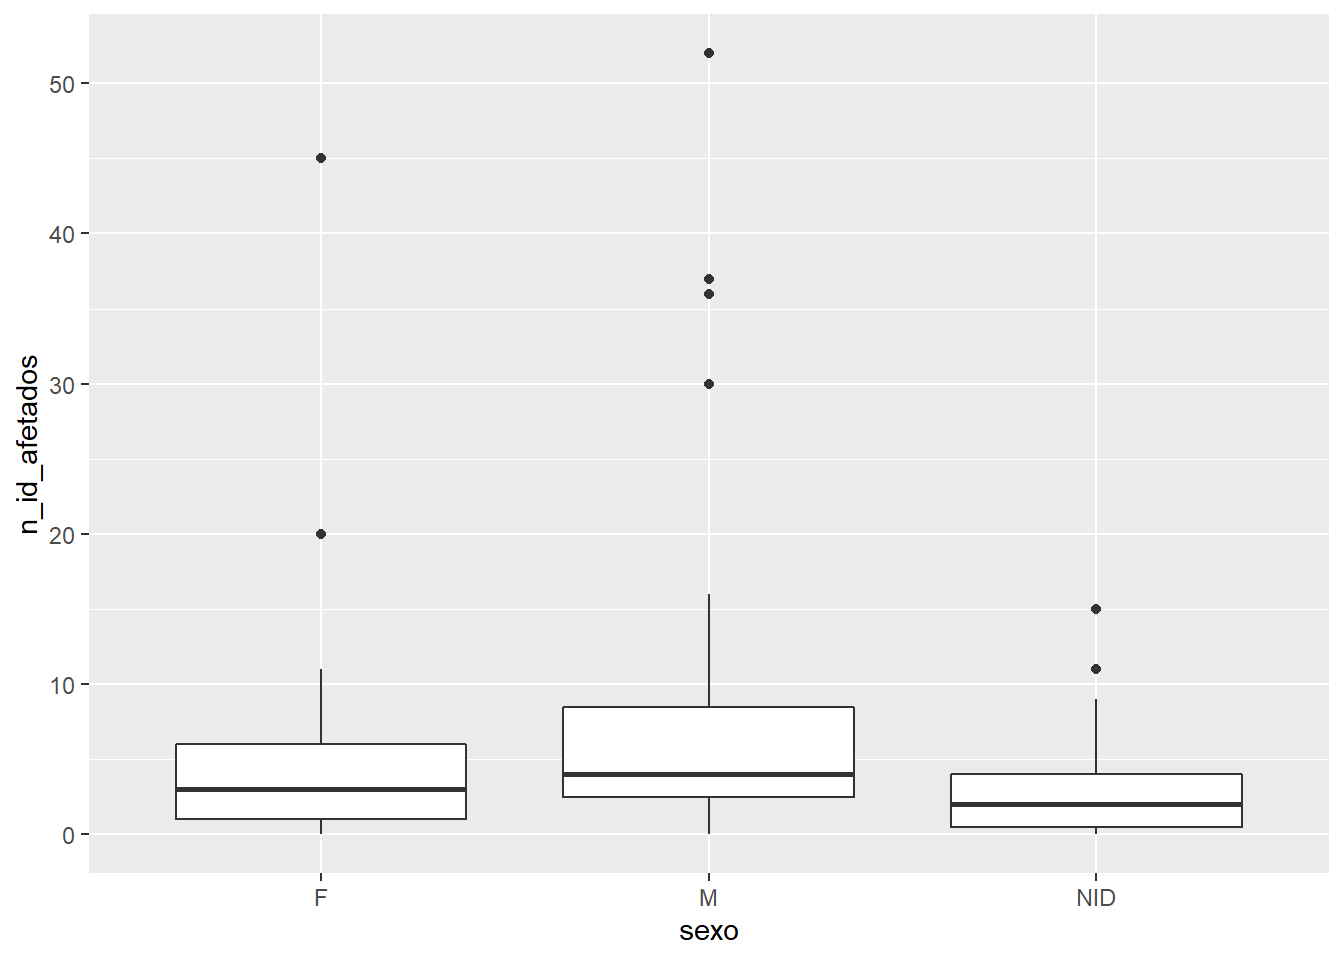
\includegraphics{data.trauma.explorer_files/figure-latex/unnamed-chunk-12-1.pdf}

\begin{Shaded}
\begin{Highlighting}[]
\FunctionTok{names}\NormalTok{(data.tr.peru)}
\end{Highlighting}
\end{Shaded}

\begin{verbatim}
##  [1] "autor_ano"               "pais"                   
##  [3] "regiao"                  "sitio"                  
##  [5] "long_leste_m"            "lat_sul_m"              
##  [7] "elevacao_m"              "cultura"                
##  [9] "cronologia"              "data_absBP_.inicial"    
## [11] "data_absBP_final"        "sexo"                   
## [13] "n_id"                    "n_id_traumas"           
## [15] "sem_traumas"             "fr_traumas"             
## [17] "n_id_antimortem"         "fr_antimortem"          
## [19] "n_id_perimortem"         "fr_perimortem"          
## [21] "n_tr_anterior"           "nasal"                  
## [23] "frontal"                 "n_tr_posterior"         
## [25] "n_tr_pariental"          "parietal_e"             
## [27] "pariental_d"             "n_tr_lateral"           
## [29] "n_antimortem_lateral"    "n_tr_perimortem_lateral"
## [31] "lateral_e"               "lateral_d"              
## [33] "ev_fort"                 "estr_sociopolitica"     
## [35] "clima"                   "carc_geografica"
\end{verbatim}

\begin{Shaded}
\begin{Highlighting}[]
\NormalTok{data.tr.peru }\SpecialCharTok{\%\textgreater{}\%} \FunctionTok{filter}\NormalTok{(}\SpecialCharTok{!}\FunctionTok{is.na}\NormalTok{(n\_id))}\SpecialCharTok{\%\textgreater{}\%}\NormalTok{ ggplot}\SpecialCharTok{+}\FunctionTok{geom\_boxplot}\NormalTok{(}\FunctionTok{aes}\NormalTok{(}\AttributeTok{x=}\NormalTok{regiao,}\AttributeTok{y=}\NormalTok{n\_id))}
\end{Highlighting}
\end{Shaded}

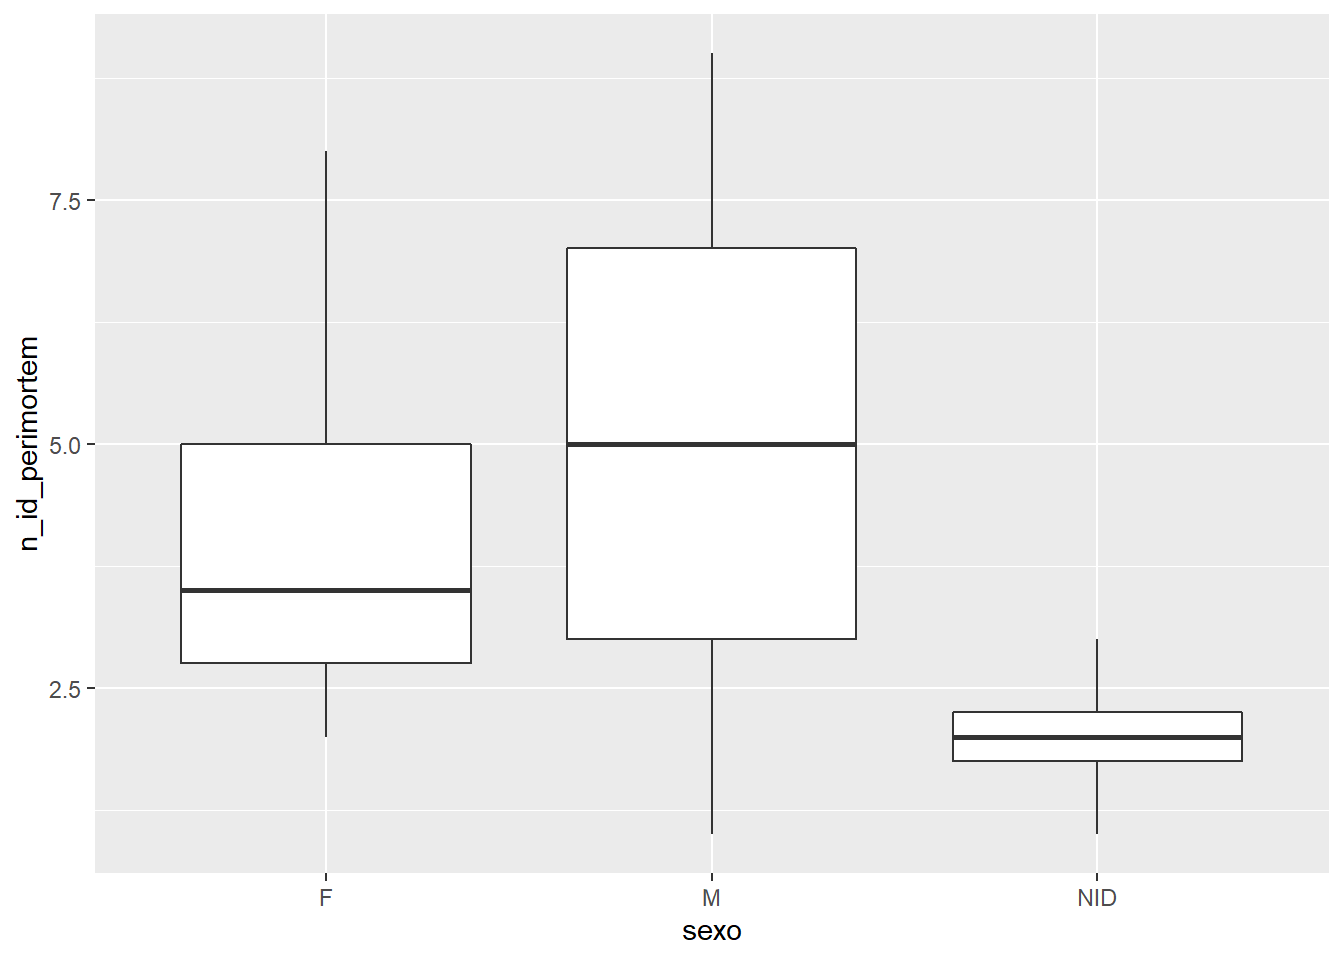
\includegraphics{data.trauma.explorer_files/figure-latex/unnamed-chunk-14-1.pdf}

\begin{Shaded}
\begin{Highlighting}[]
\NormalTok{data.tr.peru }\SpecialCharTok{\%\textgreater{}\%} \FunctionTok{filter}\NormalTok{(}\SpecialCharTok{!}\FunctionTok{is.na}\NormalTok{(n\_id\_traumas))}\SpecialCharTok{\%\textgreater{}\%}\NormalTok{ ggplot}\SpecialCharTok{+}\FunctionTok{geom\_boxplot}\NormalTok{(}\FunctionTok{aes}\NormalTok{(}\AttributeTok{x=}\NormalTok{regiao,}\AttributeTok{y=}\NormalTok{n\_id\_traumas))}
\end{Highlighting}
\end{Shaded}

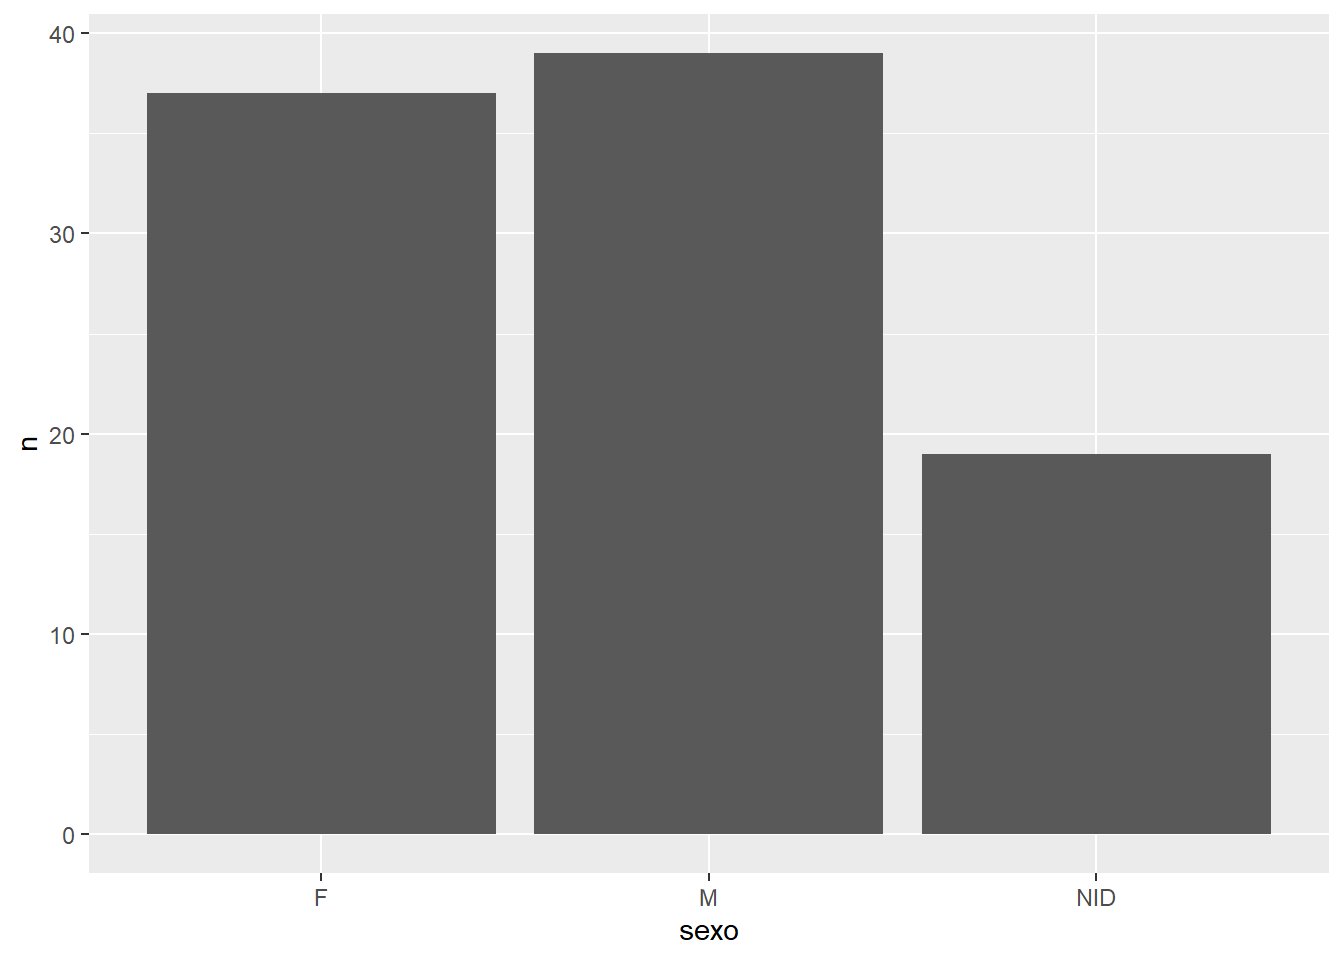
\includegraphics{data.trauma.explorer_files/figure-latex/unnamed-chunk-15-1.pdf}

\begin{Shaded}
\begin{Highlighting}[]
\CommentTok{\# os resultados mostram que o vale de majes concentra mais casos de traumas, no entanto, só pussui 4 observações, isso é desproporcional em relação ao restante}
\end{Highlighting}
\end{Shaded}

\begin{Shaded}
\begin{Highlighting}[]
\NormalTok{data.tr.peru }\SpecialCharTok{\%\textgreater{}\%} \FunctionTok{filter}\NormalTok{(}\SpecialCharTok{!}\FunctionTok{is.na}\NormalTok{(n\_id\_antimortem))}\SpecialCharTok{\%\textgreater{}\%}\NormalTok{ ggplot}\SpecialCharTok{+}\FunctionTok{geom\_boxplot}\NormalTok{(}\FunctionTok{aes}\NormalTok{(}\AttributeTok{x=}\NormalTok{regiao,}\AttributeTok{y=}\NormalTok{n\_id\_antimortem))}
\end{Highlighting}
\end{Shaded}

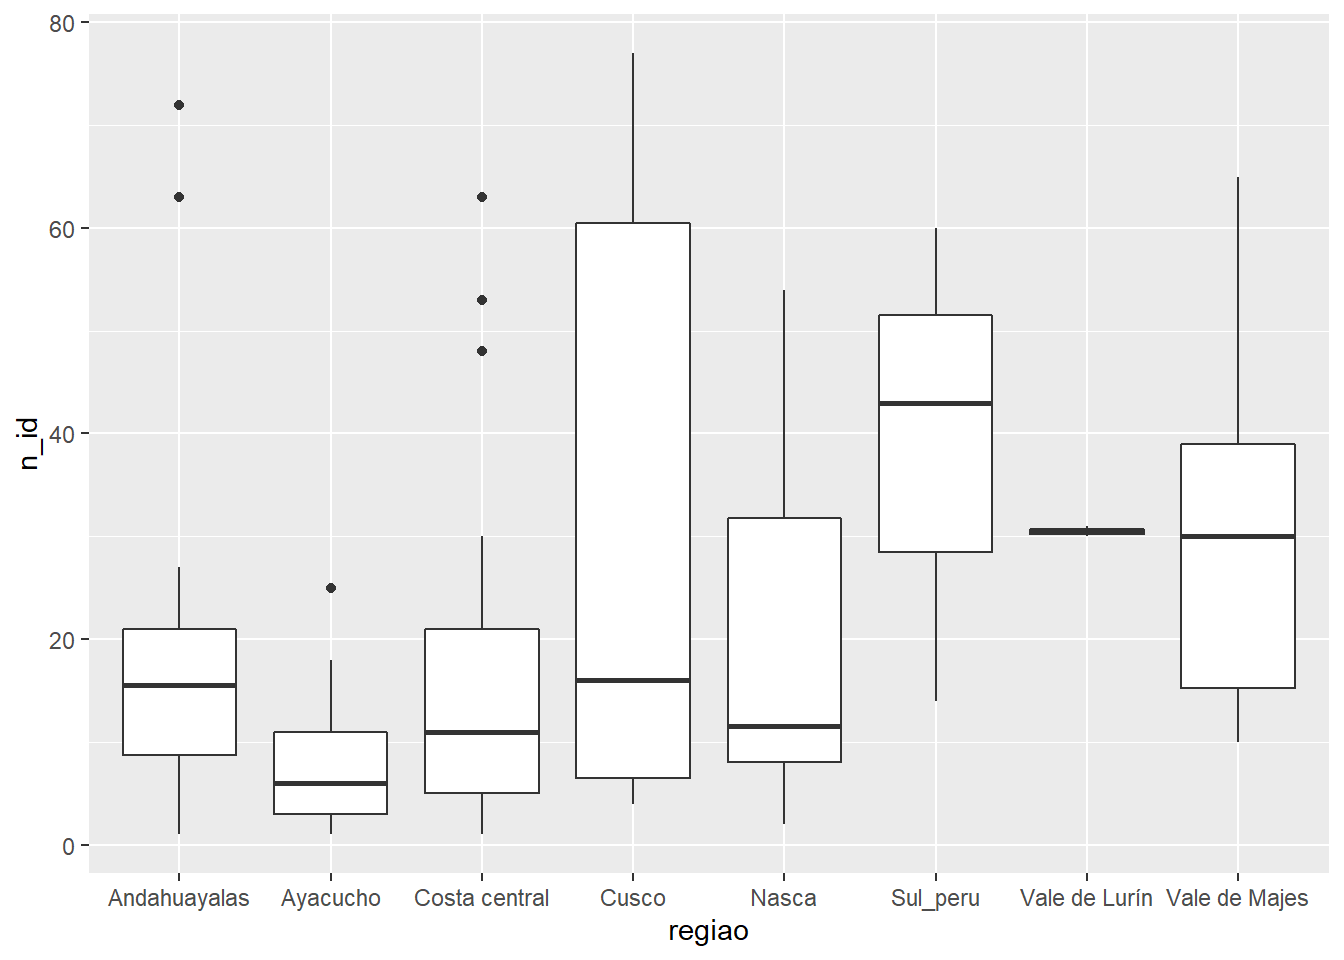
\includegraphics{data.trauma.explorer_files/figure-latex/unnamed-chunk-16-1.pdf}

\begin{Shaded}
\begin{Highlighting}[]
\NormalTok{data.tr.peru }\SpecialCharTok{\%\textgreater{}\%} \FunctionTok{filter}\NormalTok{(}\SpecialCharTok{!}\FunctionTok{is.na}\NormalTok{(n\_id\_perimortem))}\SpecialCharTok{\%\textgreater{}\%}\NormalTok{ ggplot}\SpecialCharTok{+}\FunctionTok{geom\_boxplot}\NormalTok{(}\FunctionTok{aes}\NormalTok{(}\AttributeTok{x=}\NormalTok{regiao,}\AttributeTok{y=}\NormalTok{n\_id\_perimortem))}
\end{Highlighting}
\end{Shaded}

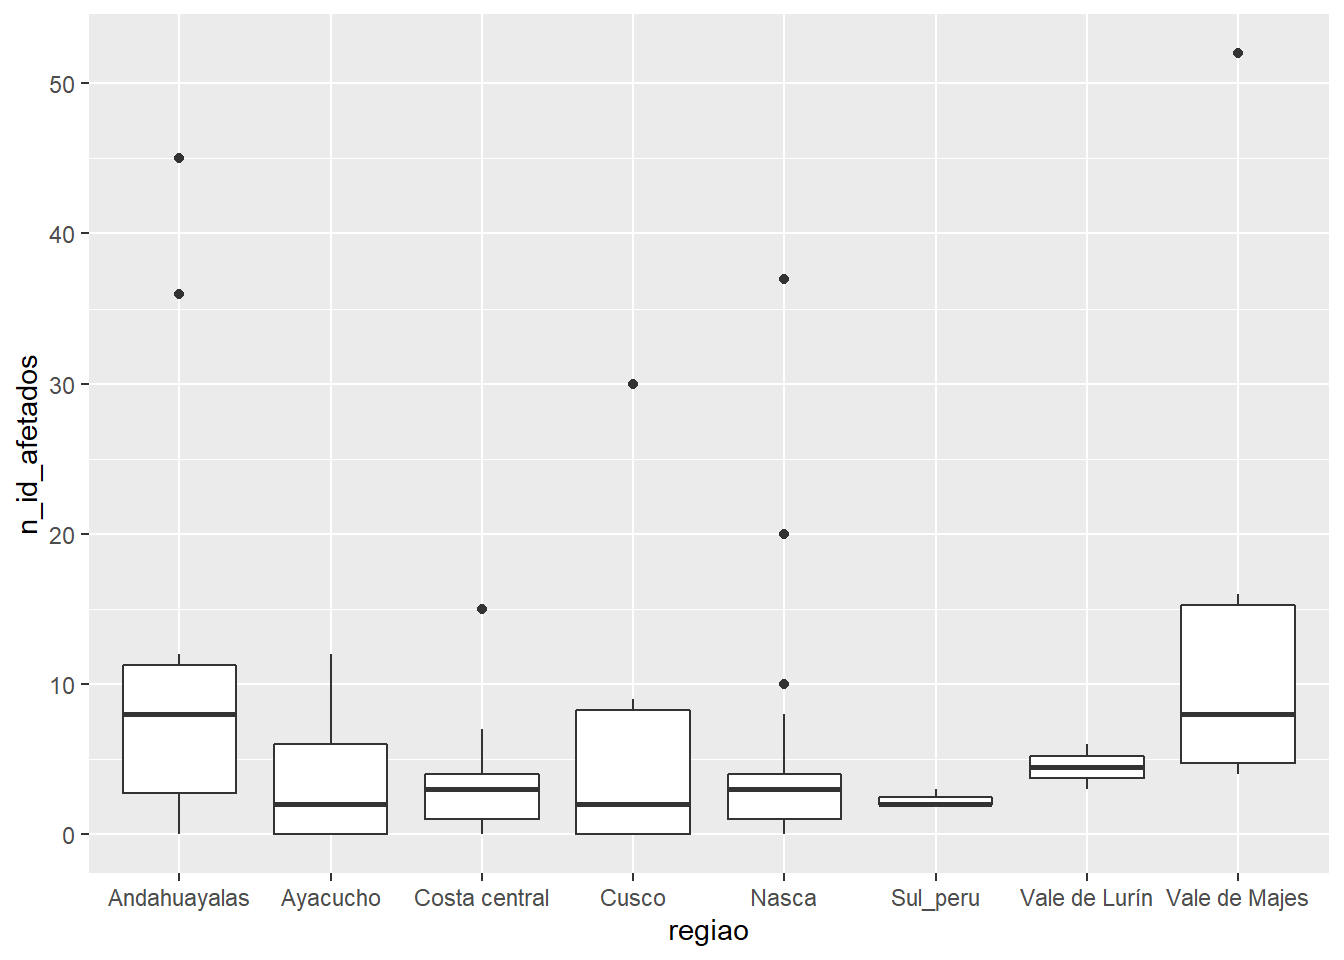
\includegraphics{data.trauma.explorer_files/figure-latex/unnamed-chunk-17-1.pdf}

Testando a associação entre as variaveis pelo teste Chiquadrado. Os
dados foram previamente preparados em forma de tabelas de contigencia
para permitir a aplicação do teste:

\begin{Shaded}
\begin{Highlighting}[]
\CommentTok{\#carregando dados em tabela de contigencia para aplicar o chiquadrado}

\CommentTok{\#por região}
\NormalTok{regiao }\OtherTok{\textless{}{-}} \FunctionTok{read.csv}\NormalTok{(}\StringTok{"regiao\_contigent.csv"}\NormalTok{, }\AttributeTok{sep =} \StringTok{";"}\NormalTok{,}\AttributeTok{row.names =} \DecValTok{1}\NormalTok{) }\SpecialCharTok{\%\textgreater{}\%} \FunctionTok{slice}\NormalTok{(}\SpecialCharTok{{-}}\DecValTok{3}\NormalTok{)  }\CommentTok{\#usando a função slice para retirar as linhas 3 correspondente a região do vale de lurin que não possui dados pareados }
\FunctionTok{View}\NormalTok{(regiao)}
\CommentTok{\#por região e sexo:}
\NormalTok{regiao\_sexo }\OtherTok{\textless{}{-}} \FunctionTok{read.csv}\NormalTok{(}\StringTok{"regiao\_sexo\_contigent.csv"}\NormalTok{, }\AttributeTok{sep =} \StringTok{";"}\NormalTok{, }\AttributeTok{row.names =} \DecValTok{1}\NormalTok{) }\SpecialCharTok{\%\textgreater{}\%} \FunctionTok{slice}\NormalTok{(}\SpecialCharTok{{-}}\DecValTok{6}\NormalTok{,}\SpecialCharTok{{-}}\DecValTok{7}\NormalTok{,}\SpecialCharTok{{-}}\DecValTok{8}\NormalTok{) }\CommentTok{\#usando a função slice para retirar as linhas 7 e 8 correspondente a região do vale de lurin que não possui dados pareados por sexo}
\FunctionTok{View}\NormalTok{(regiao\_sexo)}

\CommentTok{\#por periodo}
\NormalTok{periodo }\OtherTok{\textless{}{-}} \FunctionTok{read.csv}\NormalTok{(}\StringTok{"periodo\_contigent.csv"}\NormalTok{, }\AttributeTok{sep =} \StringTok{";"}\NormalTok{)}
\FunctionTok{View}\NormalTok{(periodo)}

\CommentTok{\#por periodo e sexo:}
\end{Highlighting}
\end{Shaded}

Aplicando Chiquadrado e visualizações gráficas das relações entre
variáveis

\begin{Shaded}
\begin{Highlighting}[]
\CommentTok{\#analisando dados de região por sítio:}

\FunctionTok{library}\NormalTok{(}\StringTok{"gplots"}\NormalTok{) }\CommentTok{\#usando o pacote de visualização dos dados matricial}
\end{Highlighting}
\end{Shaded}

\begin{verbatim}
## Warning: package 'gplots' was built under R version 4.1.3
\end{verbatim}

\begin{verbatim}
## 
## Attaching package: 'gplots'
\end{verbatim}

\begin{verbatim}
## The following object is masked from 'package:stats':
## 
##     lowess
\end{verbatim}

\begin{Shaded}
\begin{Highlighting}[]
\CommentTok{\#selecionando apenas as  colunas de número de amostras, traumas e sem traumas (há ausencia de dados nas variáveis antimortem e perimortem) e  convertendo dados em matriz:}

\NormalTok{regiao\_sexo\_at }\OtherTok{\textless{}{-}}\NormalTok{ regiao\_sexo }\SpecialCharTok{\%\textgreater{}\%} \FunctionTok{select}\NormalTok{(n\_id\_traumas,sem\_traumas)}

\NormalTok{rg.sexo.matriz }\OtherTok{\textless{}{-}} \FunctionTok{as.table}\NormalTok{(}\FunctionTok{as.matrix}\NormalTok{(regiao\_sexo\_at))}

\CommentTok{\#plotando gráfico balloonplot }

\FunctionTok{balloonplot}\NormalTok{(}\FunctionTok{t}\NormalTok{(rg.sexo.matriz), }\AttributeTok{main =}\StringTok{"região por sexo"}\NormalTok{, }\AttributeTok{xlab =}\StringTok{""}\NormalTok{, }\AttributeTok{ylab=}\StringTok{""}\NormalTok{,}
            \AttributeTok{label =} \ConstantTok{FALSE}\NormalTok{, }\AttributeTok{show.margins =} \ConstantTok{FALSE}\NormalTok{)}
\end{Highlighting}
\end{Shaded}

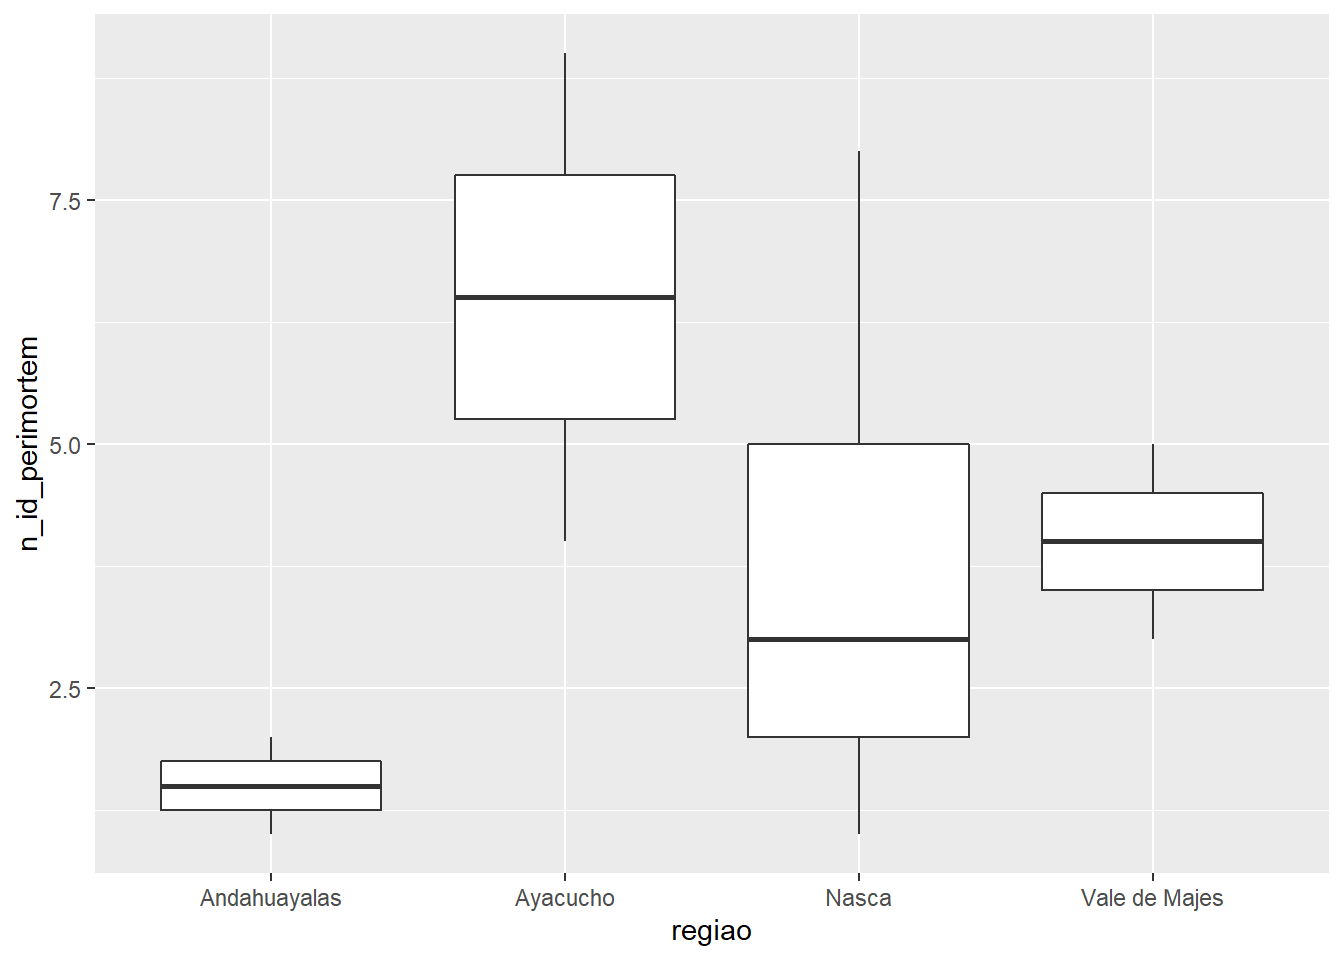
\includegraphics{data.trauma.explorer_files/figure-latex/unnamed-chunk-19-1.pdf}

\begin{Shaded}
\begin{Highlighting}[]
\CommentTok{\#aplicando teste chiquadrado para independencia das amostras}
\NormalTok{chisq }\OtherTok{\textless{}{-}} \FunctionTok{chisq.test}\NormalTok{(rg.sexo.matriz)}
\NormalTok{chisq}
\end{Highlighting}
\end{Shaded}

\begin{verbatim}
## 
##  Pearson's Chi-squared test
## 
## data:  rg.sexo.matriz
## X-squared = 68.936, df = 9, p-value = 2.461e-11
\end{verbatim}

\begin{Shaded}
\begin{Highlighting}[]
\NormalTok{periodo\_sexo }\OtherTok{\textless{}{-}}\FunctionTok{read.csv}\NormalTok{(}\StringTok{"periodo\_sexo\_contigent.csv"}\NormalTok{, }\AttributeTok{sep =} \StringTok{";"}\NormalTok{, }\AttributeTok{row.names =} \DecValTok{1}\NormalTok{)}\CommentTok{\#row.names = 1) \%\textgreater{}\% select(n\_id,n\_id\_traumas,sem\_traumas) \%\textgreater{}\% slice({-}6)}
\FunctionTok{names}\NormalTok{(periodo\_sexo)}
\end{Highlighting}
\end{Shaded}

\begin{verbatim}
## [1] "n_id"            "n_id_traumas"    "sem_traumas"     "n_id_antimortem"
## [5] "n_id_perimortem"
\end{verbatim}

\begin{Shaded}
\begin{Highlighting}[]
\CommentTok{\#View(periodo\_sexo)}
\FunctionTok{head}\NormalTok{(periodo\_sexo)}
\end{Highlighting}
\end{Shaded}

\begin{verbatim}
##         n_id n_id_traumas sem_traumas n_id_antimortem n_id_perimortem
## HM_F      30            6          24               6               0
## HM_M      90           58          32              54               5
## HM_NID   182           60         122              51               6
## PIP_F     35            5          30               2               0
## PIP_M     31            7          24               1               0
## PIP_NID    6            0           6               0               0
\end{verbatim}

\begin{Shaded}
\begin{Highlighting}[]
\NormalTok{periodo\_sexo\_at }\OtherTok{\textless{}{-}}\NormalTok{ periodo\_sexo }\SpecialCharTok{\%\textgreater{}\%} \FunctionTok{select}\NormalTok{(n\_id\_traumas,sem\_traumas)}

\NormalTok{pr.sexo.matriz }\OtherTok{\textless{}{-}} \FunctionTok{as.table}\NormalTok{(}\FunctionTok{as.matrix}\NormalTok{(periodo\_sexo\_at))}

\CommentTok{\#plotando gráfico balloonplot }

\FunctionTok{balloonplot}\NormalTok{(}\FunctionTok{t}\NormalTok{(pr.sexo.matriz), }\AttributeTok{main =}\StringTok{"período por sexo"}\NormalTok{, }\AttributeTok{xlab =}\StringTok{""}\NormalTok{, }\AttributeTok{ylab=}\StringTok{""}\NormalTok{,}
            \AttributeTok{label =} \ConstantTok{FALSE}\NormalTok{, }\AttributeTok{show.margins =} \ConstantTok{FALSE}\NormalTok{)}
\end{Highlighting}
\end{Shaded}

\includegraphics{data.trauma.explorer_files/figure-latex/unnamed-chunk-22-1.pdf}

\begin{Shaded}
\begin{Highlighting}[]
\CommentTok{\#aplicando teste chiquadrado para independencia das amostras}
\NormalTok{chisq }\OtherTok{\textless{}{-}} \FunctionTok{chisq.test}\NormalTok{(pr.sexo.matriz)}
\end{Highlighting}
\end{Shaded}

\begin{verbatim}
## Warning in chisq.test(pr.sexo.matriz): Chi-squared approximation may be
## incorrect
\end{verbatim}

\begin{Shaded}
\begin{Highlighting}[]
\NormalTok{chisq}
\end{Highlighting}
\end{Shaded}

\begin{verbatim}
## 
##  Pearson's Chi-squared test
## 
## data:  pr.sexo.matriz
## X-squared = 84.425, df = 8, p-value = 6.263e-15
\end{verbatim}

Aplicando teste Kruskal-Wallis (TÁ ERRADO, CONCERTA)

\begin{Shaded}
\begin{Highlighting}[]
\NormalTok{periodo.sexo.kw }\OtherTok{\textless{}{-}}\FunctionTok{read.csv}\NormalTok{(}\StringTok{"periodo\_sexo\_contigent.csv"}\NormalTok{, }\AttributeTok{sep =} \StringTok{";"}\NormalTok{)}\CommentTok{\#, stringsAsFactors = TRUE) \%\textgreater{}\% slice({-}6)}

\CommentTok{\#levels(periodo.sexo.kw$Periodo)}

\FunctionTok{kruskal.test}\NormalTok{(Periodo }\SpecialCharTok{\textasciitilde{}}\NormalTok{ n\_id\_traumas , }\AttributeTok{data=}\NormalTok{ periodo.sexo.kw)}
\end{Highlighting}
\end{Shaded}

\begin{verbatim}
## 
##  Kruskal-Wallis rank sum test
## 
## data:  Periodo by n_id_traumas
## Kruskal-Wallis chi-squared = 8, df = 8, p-value = 0.4335
\end{verbatim}

\begin{Shaded}
\begin{Highlighting}[]
\CommentTok{\#levels(periodo\_sexo\_at$)}
\end{Highlighting}
\end{Shaded}

\begin{Shaded}
\begin{Highlighting}[]
\FunctionTok{kruskal.test}\NormalTok{(n\_id\_antimortem }\SpecialCharTok{\textasciitilde{}}\NormalTok{ Periodo, }\AttributeTok{data=}\NormalTok{ periodo.sexo.kw)}
\end{Highlighting}
\end{Shaded}

\begin{verbatim}
## 
##  Kruskal-Wallis rank sum test
## 
## data:  n_id_antimortem by Periodo
## Kruskal-Wallis chi-squared = 8, df = 8, p-value = 0.4335
\end{verbatim}

\begin{Shaded}
\begin{Highlighting}[]
\FunctionTok{kruskal.test}\NormalTok{(n\_id\_perimortem }\SpecialCharTok{\textasciitilde{}}\NormalTok{ Periodo, }\AttributeTok{data=}\NormalTok{ periodo.sexo.kw)}
\end{Highlighting}
\end{Shaded}

\begin{verbatim}
## 
##  Kruskal-Wallis rank sum test
## 
## data:  n_id_perimortem by Periodo
## Kruskal-Wallis chi-squared = 8, df = 8, p-value = 0.4335
\end{verbatim}

\begin{Shaded}
\begin{Highlighting}[]
\FunctionTok{kruskal.test}\NormalTok{(n\_id }\SpecialCharTok{\textasciitilde{}}\NormalTok{ Periodo, }\AttributeTok{data=}\NormalTok{ periodo.sexo.kw)}
\end{Highlighting}
\end{Shaded}

\begin{verbatim}
## 
##  Kruskal-Wallis rank sum test
## 
## data:  n_id by Periodo
## Kruskal-Wallis chi-squared = 8, df = 8, p-value = 0.4335
\end{verbatim}

\begin{Shaded}
\begin{Highlighting}[]
\FunctionTok{pairwise.wilcox.test}\NormalTok{(periodo.sexo.kw}\SpecialCharTok{$}\NormalTok{n\_id\_traumas,periodo.sexo.kw}\SpecialCharTok{$}\NormalTok{Periodo)}
\end{Highlighting}
\end{Shaded}

\begin{verbatim}
## 
##  Pairwise comparisons using Wilcoxon rank sum exact test 
## 
## data:  periodo.sexo.kw$n_id_traumas and periodo.sexo.kw$Periodo 
## 
##         HM_F HM_M HM_NID PIP_F PIP_M PIP_NID PIT_F PIT_M
## HM_M    1    -    -      -     -     -       -     -    
## HM_NID  1    1    -      -     -     -       -     -    
## PIP_F   1    1    1      -     -     -       -     -    
## PIP_M   1    1    1      1     -     -       -     -    
## PIP_NID 1    1    1      1     1     -       -     -    
## PIT_F   1    1    1      1     1     1       -     -    
## PIT_M   1    1    1      1     1     1       1     -    
## PIT_NID 1    1    1      1     1     1       1     1    
## 
## P value adjustment method: holm
\end{verbatim}

\begin{Shaded}
\begin{Highlighting}[]
\CommentTok{\# p.adjust.method ="BH")}
\end{Highlighting}
\end{Shaded}


\end{document}
